\documentclass{article}

% NeurIPS styling
\usepackage[preprint,nonatbib]{neurips_2024}

\usepackage[utf8]{inputenc}
\usepackage{lmodern}
\usepackage{hyperref}
\usepackage{url}
\usepackage{booktabs}
\usepackage{amsfonts}
\usepackage{nicefrac}
\usepackage{microtype}
\usepackage{xcolor}
\usepackage{graphicx}
\usepackage{caption}

\title{A Comparative Analysis of Edge Native Vision Language Model Architectures for Autonomous Decision Support in Asset Integrity Management in Industries}

\author{
  Anonymous Authors \\
  NeurIPS 2024 Submission \\
}

\begin{document}
\maketitle

\begin{abstract}
Oil and gas plants still use legacy analog gauges and pipelines requiring manual inspection. Replacing them with networked digital sensors is financially unviable. Offline Vision Language Models (VLMs) offer a potential retrofit solution. Existing benchmarks test general visual question answering rather than industrial Standard Operating Procedure (SOP) compliance under constrained edge memory environments. We evaluate six edge-native VLMs with fewer than three billion parameters using a custom dual-rule dataset designed to measure strict logic compliance over default visual priors. Across 15,000 evaluations, we test zero-shot accuracy against prompt decomposition and dual-channel CLAHE optical preprocessing. McNemar’s testing proves that forcing step-by-step logic actively degrades some baseline architectures while rescuing others. Imposing text constraints triggers total modality collapse in SmolVLM. Its false negative rate hits 100 percent. Janus breaks format entirely and generates 115 unparseable outputs. Applying the exact same constraints to Qwen2-VL prevents baseline failure. Unified models like Gemma 4 ignore optical contrast enhancements. Attempting to cure modality collapse via Parameter-Efficient Fine-Tuning (LoRA) causes Optimization Saturation. Restoring logic compliance requires structural optical grounding through Agentic Foveation. Our results categorize the engineering trade-offs required for scaling VLMs for offline industrial audits.
\end{abstract}


\section*{Introduction}


\textbf{[Proposed Figure 1: Horizontal Evaluation Pipeline Diagram]}
\textit{(To be generated externally - see prompt provided)}

Industrial environments, such as oil refineries and chemical plants, depend on thousands of legacy analog gauges and complex pipeline manifolds to monitor systemic health. Automating the supervision of these physical assets remains a critical bottleneck in facility maintenance. Replacing every analog gauge with a networked digital sensor is technically possible, but the scale of legacy infrastructure renders this approach cost-prohibitive. Vision Language Models offer a retrofit solution by extracting operational states directly from simple camera feeds. Cloud-based application programming interfaces (APIs) provide massive computational capacity. Industrial auditing prohibits their use. Remote sites suffer from latency, unreliable internet connectivity, and severe data privacy regulations surrounding proprietary infrastructure. Auditing systems must run locally on-device. Deploying server-grade models holding billions of parameters to remote edges creates immediate hardware barriers. Remote edge server environments throttle available memory bandwidth, making standard massive architectures computationally impractical. This hardware ceiling dictates a need to validate the industrial capabilities of high-efficiency models designed to operate near the three-billion parameter boundary without extreme, unstable compression frameworks.

Existing benchmarks for edge-native Vision Language Models evaluate generalized visual question answering or simple optical character recognition. These generalized metrics do not translate to safe industrial deployment. In high-risk environments, transcribing a gauge dial is insufficient. An autonomous auditing system must extract the visual reading, compare it against a strict boundary condition defined by a Standard Operating Procedure, and output a tightly constrained logic verdict. When unproven models encounter these multi-constraint logic tasks, they frequently abandon the visual evidence entirely. 

This processing bottleneck creates a critical safety hazard: pleasing bias. When a small-scale model lacks the capacity to simultaneously process the image array and the complex text rules, it defaults to its training distribution. Instead of alerting operators to an out-of-bounds anomaly or admitting an inability to read the dial, the model confidently outputs a normal, safe operational state. Relying on baseline capability without benchmarking industrial rule adherence actively risks disastrous false negatives, allowing physical mechanical failures to go unnoticed. The evaluation baseline must shift from measuring generalized perception to explicitly measuring logic instruction compliance.

We map this functional baseline by testing the exact failure boundaries of six prominent edge-native Vision Language Models: SmolVLM, Janus, InternVL2, Gemma 4, Qwen2-VL, and MiniCPM. We subject these architectures to a constrained test matrix isolating strict logic adherence from unconstrained zero-shot perception. By executing an exhaustive zero-shot baseline alongside explicit text-based and optical interventions, we map the hardware point where structural prompt formatting overrides visual perception.

Our primary contributions are:
\begin{itemize}
    \item We introduce the Golden 100 Benchmark, an evaluation framework pairing analog industrial imagery with conflicting dual-rule logic protocols to measure strict conditional reasoning.
    \item We define the Formatting Penalty boundary. McNemar's testing proves that imposing structural logic constraints (Chain-of-Thought) induces complete modality collapse in smaller architectures but prevents failure in larger decoupled architectures.
    \item We demonstrate through Parameter-Efficient Fine-Tuning (LoRA) that adapting the visual encoder and multimodal projector fails to cure Modality Collapse. The reasoning bottleneck in sub-3B architectures is fundamentally linguistic rather than strictly visual.
    \item We introduce Agentic Foveation, an automated spatial-cropping pipeline that bypasses the hardware token-density ceiling. By algorithmically forcing the physical anomaly to dominate the context window, we provide a deployable mechanism for restoring logic compliance in hardware-constrained edge environments.
\end{itemize}


\section*{Related Work}


\subsection*{The Shift to Edge-Native Architectures}

Modern industrial plants cannot rely on cloud-based Vision-Language Models (VLMs) due to strict data privacy regulations and unstable network latency. This strictness forces researchers to compress visual reasoning capabilities into hardware-constrained environments. Frontier models like GPT-4o and InternVL (40B) set performance benchmarks but remain physically non-deployable at the edge. Development has pivoted toward sub-3B parameter architectures designed specifically for local execution. SmolVLM reduces memory footprints using aggressive pixel-shuffle compression [2]. MiniCPM-V-2.0 pushes high-tier reasoning benchmarks down into a highly efficient 2.8B parameter envelope [1]. Compressing a neural architecture inherently sacrifices its structural logic capacity. These edge models excel at simple image captioning tasks. Their reliability remains unproven when deployed into high-stakes safety auditing loops requiring rigid, multi-step rule evaluation.

\subsection*{Modality Collapse in Vision-Language Processing}

Deploying compressed architectures into safety loops introduces a primary danger: they ignore physical visual evidence. When complex logic constraints overwhelm a model's parameterized memory, it reverts to the dominant linguistic patterns encountered during pre-training. This phenomenon is Modality Collapse. It occurs when a model outputs a statistically probable text response rather than analyzing the provided image tensor. The MM-SHAP framework mathematically confirms that unconstrained models seek these linguistic shortcuts when faced with visual ambiguity [3]. Evaluation methods like ROPE demonstrate that in cluttered scenes, hallucination rates scale with the entropy of the text tokens rather than physical visual cues [4]. In an industrial context, a VLM guessing that a pipeline gauge reads normal because normal is a frequent training label represents a catastrophic auditing failure.

\subsection*{Prompting Constraints and The Formatting Penalty}

Engineers typically implement rigid prompting structures like step-by-step Chain-of-Thought (CoT) to prevent Modality Collapse and force models to analyze physics. Imposing structured logic introduces a secondary failure mode: the formatting penalty. Benchmarks such as MeasureBench illustrate that smaller language models often fail a task because they cannot adhere to strict parsing boundaries or structural markers [5]. High-parameter models possess the attention capacity to simultaneously evaluate a visual scene and follow complex parsing rules using a Holistic-Thought Protocol [6]. Edge models lack this dual capacity. When forced to process visual anomalies while adhering to strict syntax protocols, sub-3B models trigger linguistic recursion loops. An effective industrial VLM comparison must evaluate visual accuracy and the specific breaking point where strict formatting constraints cause the architecture to fail.

\subsection*{Parameter-Efficient Fine-Tuning and Visual Grounding}

When prompt engineering fails, developers turn to Parameter-Efficient Fine-Tuning (PEFT), such as Low-Rank Adaptation (LoRA) [22], to hardcode task-specific behaviors without catastrophic forgetting. LoRA excels at format adherence and style transfer. Recent research indicates it struggles to inject new fundamental reasoning pathways into highly constrained parameter spaces, leading to Optimization Saturation [23]. To bypass the linguistic formatting penalty and the limits of PEFT, alternative approaches rely on visual spatial grounding. Techniques like foveation algorithmically crop the input tensor to isolate high-relevance pixels, inspired by the zero-shot spatial isolation capabilities of foundation models like Segment Anything (SAM) [24]. This physically forces the attention mechanism to center on visual evidence rather than broad semantic context. This limits the total token density the architecture must process, relieving cognitive load during complex logical evaluations.


\section*{Methodology}


\subsection*{The "Golden 100" Benchmark and Constraint Injection}

Standard Vision-Language benchmarks evaluate generalized reasoning capacity by probing spatial adherence like VALSE and Winoground [7, 8]. This methodology measures industrial logic adherence. We curated a "Golden 100" dataset of extreme physical edge cases to prevent models from relying on generalized pre-training. We aggregated raw images from open-source Roboflow datasets: 50 analog gauges from the `gauge-kzdux` dataset, and 50 structural pipeline images equally from the `Classi1` and `Non-Corroded-Pipe` datasets [19, 20, 21]. We rejected automated scraping. Human annotators manually selected the images and provided ground-truth readings, ensuring a perfect split between defective anomalies and clean controls. We tagged each image for specific visual stressors, including oblique angles, specular glare, low contrast, and structural obstructions.

To audit conditional inference rather than visual guessing, we implemented a "Constraint Injection" test inspired by LogicQA and LogicAD [9, 10]. We synthesized the 100 unique images into a 200-row inference matrix by assigning each image two mutually exclusive Standard Operating Procedures (SOPs). Rule A dictates that any surface oxidation triggers an alert (`UNSAFE`). Rule B provides a lenient limit where surface rust is normal (`SAFE`). True logic compliance requires the model to reverse its verdict on the exact same physical image tensor because the text-based SOP changed.

\subsection*{Dual-Channel Optical Resolution and CLAHE Integration}

Industrial sub-3B architectures operate under extreme hardware-imposed pixel compression limits. High-resolution input tensors natively downscale to strict low-resolution tensor caps (e.g., 336px to 384px) to fit VRAM bandwidths. This optical crushing amplifies ambient lighting noise, turning minor shadows or glass glare into opaque physical artifacts that permanently obscure gauge pointers. We implemented a dual-channel testing pipeline using Contrast Limited Adaptive Histogram Equalization (CLAHE) to computationally enhance the raw inputs [14]. This isolates whether models failed on logic or strictly due to structural pixel crush. Maximizing local spatial contrast before the compression boundary allowed us to isolate the hardware pixel bottleneck from the inherent logic capacity of the models.

\subsection*{Broad Architectural Evaluation}

We evaluated the logic breakdown threshold across an escalating inference matrix to map the baseline failure points of all six models. We implemented the following structured interventions:
\begin{enumerate}
    \item \textbf{Zero-Shot Baseline:} We tested the models by providing the raw image and the full safety rule in a single prompt. This establishes the base failure rate before cognitive scaffolding.
    \item \textbf{Chain-of-Thought (CoT):} We forced the models to outline their step-by-step logic before rendering a final verdict. The goal was to determine if sequential reasoning prevents Modality Collapse. Recent literature indicates that imposing strict syntax without targeted training data triggers the formatting penalty in sub-3B models [13].
    \item \textbf{Rule Decomposition:} To bypass the linguistic formatting penalty observed in CoT, we decomposed the complex safety rule into separate, sequential binary checks (e.g., "Is there a needle?", followed by "Is it pointing past the red line?"). This reduced the concurrent token load the architecture had to process.
    \item \textbf{Contrast with Decomposition:} We merged the optically enhanced CLAHE images with the sequential binary checks of Rule Decomposition to isolate whether the failure was visual or logical. We initially tested CLAHE alongside standard CoT, but the formatting penalty persisted and skewed the results. We isolated Contrast + Decomposition as the definitive "best-case scenario" to map the maximum intelligence ceiling of the models when visual noise and formatting penalties are removed.
\end{enumerate}

\subsection*{Targeted Structural Interventions (Qwen2-VL)}

We conducted two advanced interventions exclusively on Qwen2-VL to test whether structural limitations could be overcome through weight updates or spatial isolation. Qwen2-VL demonstrated the highest base resilience during our broad evaluation:

\subsubsection*{Parameter-Efficient Fine-Tuning (LoRA)}

We fine-tuned Qwen2-VL using Low-Rank Adaptation (LoRA) to natively internalize the dataset's logical structure. The goal was to determine if weight-updates cure Modality Collapse and allow the model to execute strict logic without explicit CoT prompting, bypassing the formatting penalty. To prevent degradation of the model's base language reasoning capabilities, we applied adaptation strictly to the perception layers. We targeted 3 late-stage vision encoder blocks (`visual.blocks.21-23`) and 2 multimodal projector layers (`visual.merger.mlp.0, .2`), utilizing a rank of $r=16$ and an alpha of 32.

The model trained on 800 synthetically augmented samples. To prevent data leakage, we generated these via cropping, rotation, brightness shifts, and contrast adjustments from a distinct curated training set of 100 gauge images. The Golden 100 benchmark remained strictly isolated for inference testing. We utilized a fully synced 720/80 train/validation split. Training ran over 5 epochs with an effective batch size of 8 (batch size 4, gradient accumulation 2), a learning rate of 2e-5, and a cosine learning rate scheduler. We implemented strict `-100` label masking on the system prompts and instructions. The loss function calculated exclusively on the generated gauge reading and final rule verdict. Fixed `max\_length` constraints were removed during collation to prevent the truncation of dense visual tokens produced by the high-resolution gauge images.

\subsubsection*{Agentic Foveation}

We implemented an automated spatial-cropping pipeline called Agentic Foveation to physically bypass the hardware token-density ceiling. This pipeline uses Qwen2-VL as its own spatial grounding agent, decoupling visual search from logical reasoning into three explicit stages:
\begin{enumerate}
    \item \textbf{Spatial Localization:} The prompt asks the model to generate a brief textual description of where the primary region of interest is located (e.g., "centre", "upper-left"), and then output a tight bounding box using normalized `[0, 1000]` coordinates. This intermediate descriptive step acts as a spatial Chain-of-Thought, anchoring the model's attention before it predicts raw integer coordinates.
    \item \textbf{Foveated Cropping and Upscaling:} The original high-resolution image tensor physically crops to the model's generated coordinates with an added 15\% padding margin to preserve edge context. This cropped region forcefully upscales to $1024 \times 1024$ pixels. 
    \item \textbf{Targeted Reasoning:} This high-resolution, isolated crop passes back to the model for a second inference pass to evaluate the logical safety rule using \textbf{Rule Decomposition} prompting. Removing irrelevant background pixels and forcing high-density token allocation onto the anomaly frees the model's constrained attention mechanism from optical noise. This lowers the cognitive load required for strict logical evaluation.
\end{enumerate}

\subsection*{Experimental Setup and Statistical Protocol}

The pipeline bounded operations to an 8GB Total VRAM limit, achieving peak inference at 4.6 GB using 4-bit quantization. We evaluated six frontier models representing four distinct architectural approaches to vision processing:
\begin{itemize}
    \item \textbf{Projector-Based Architectures:} These models rely on an explicitly modular pipeline, represented in our framework by SmolVLM (0.6B), InternVL2 (1.0B), and MiniCPM (2.8B). They utilize a pre-trained Vision Transformer format to encode image patches into dense feature embeddings, routed through a Multi-Layer Perceptron projector into the textual latent space of the underlying language model. This structural bottleneck forces all spatial geometry and physical anomalies to translate into linguistic approximations prior to reasoning.
    \item \textbf{Decoupled Architectures:} Decoupled architectures physically separate the visual understanding pathway from the generative text pathway, as demonstrated by Janus (1.3B). By maintaining independent encoding modules, the architecture isolates the visual tensor from the disproportionate weight of the language pre-training. This protects subtle visual signals from linguistic dominance during complex logical evaluations.
    \item \textbf{Dynamic Resolution Architectures:} Represented by Qwen2-VL (2.2B), this architecture abandons fixed-patch sizing. It dynamically subdivides high-resolution inputs into variable grids, allocating denser token groupings to complex spatial regions while compressing empty space. This allows the model to process $1024 \times 1024$ equivalent details without exponentially exploding the context window.
    \item \textbf{Unified Multimodal Architectures:} Represented by Gemma-4-E2B-it (2B), natively unified architectures share the embedding space completely between visual and text tokens rather than passing visual data through a dedicated projector. This shared space makes the network highly susceptible to "Structural Modality Collapse," where underlying LLM safety or conversational priors overpower the visual signal.
\end{itemize}

Our framework enforces a three-pass evaluation protocol. Every model ran three independent physical inference passes across all five paradigm interventions, producing 9,000 recorded broad evaluations (excluding the targeted LoRA and Foveation runs on Qwen2-VL). We disabled random generation to guarantee that logic variance resulted from architectural processing limits rather than hyperparameter drift. A fault-tolerant regex compiling engine processed broken text structures, flagging syntax failures or physical hallucination loops universally as a failure to render a verdict. Significance across all paired-row cross-validations computed strictly via McNemar's Test for paired nominal data [11], executing rigorous multiple hypothesis corrections [12].


\section*{Experimental Results and Architectural Diagnostics}



\begin{table*}[t]
\centering
\caption{Comprehensive performance metrics across all sub-3B architectures and interventions. We report mean F1 Score and False Negative Rate (FNR). FNR is the critical metric for industrial safety.}
\label{tab:main_results}
\resizebox{\textwidth}{!}{%
\begin{tabular}{l|cc|cc|cc|cc|cc}
\toprule
\textbf{Model} & \multicolumn{2}{c|}{\textbf{Baseline}} & \multicolumn{2}{c|}{\textbf{CoT}} & \multicolumn{2}{c|}{\textbf{Decomp}} & \multicolumn{2}{c|}{\textbf{CLAHE + CoT}} & \multicolumn{2}{c}{\textbf{CLAHE + Decomp}} \\
& F1 $\uparrow$ & FNR $\downarrow$ & F1 $\uparrow$ & FNR $\downarrow$ & F1 $\uparrow$ & FNR $\downarrow$ & F1 $\uparrow$ & FNR $\downarrow$ & F1 $\uparrow$ & FNR $\downarrow$ \\
\midrule
\textbf{SmolVLM} & 0.444 & 0.588 & 0.000 & 1.000 & 0.018 & 0.990 & 0.000 & 1.000 & 0.024 & 0.987 \\
\textbf{InternVL2} & 0.431 & 0.702 & 0.605 & 0.314 & 0.687 & 0.231 & 0.489 & 0.486 & 0.654 & 0.181 \\
\textbf{Janus} & 0.219 & 0.865 & 0.299 & 0.807 & 0.143 & 0.919 & 0.272 & 0.823 & 0.144 & 0.915 \\
\textbf{Qwen2-VL} & 0.294 & 0.810 & 0.616 & 0.267 & 0.621 & 0.476 & 0.541 & 0.400 & 0.600 & 0.429 \\
\textbf{Gemma 4} & 0.117 & 0.933 & 0.024 & 0.987 & 0.095 & 0.949 & 0.055 & 0.971 & 0.111 & 0.940 \\
\textbf{MiniCPM} & 0.420 & 0.697 & 0.631 & 0.390 & 0.680 & 0.171 & 0.633 & 0.340 & 0.699 & 0.163 \\
\bottomrule
\end{tabular}%
}
\vspace{-0.15in}
\end{table*}



\subsection*{The Reality of Zero-Shot Modality Collapse}


\begin{figure}[htbp]
    \centering
    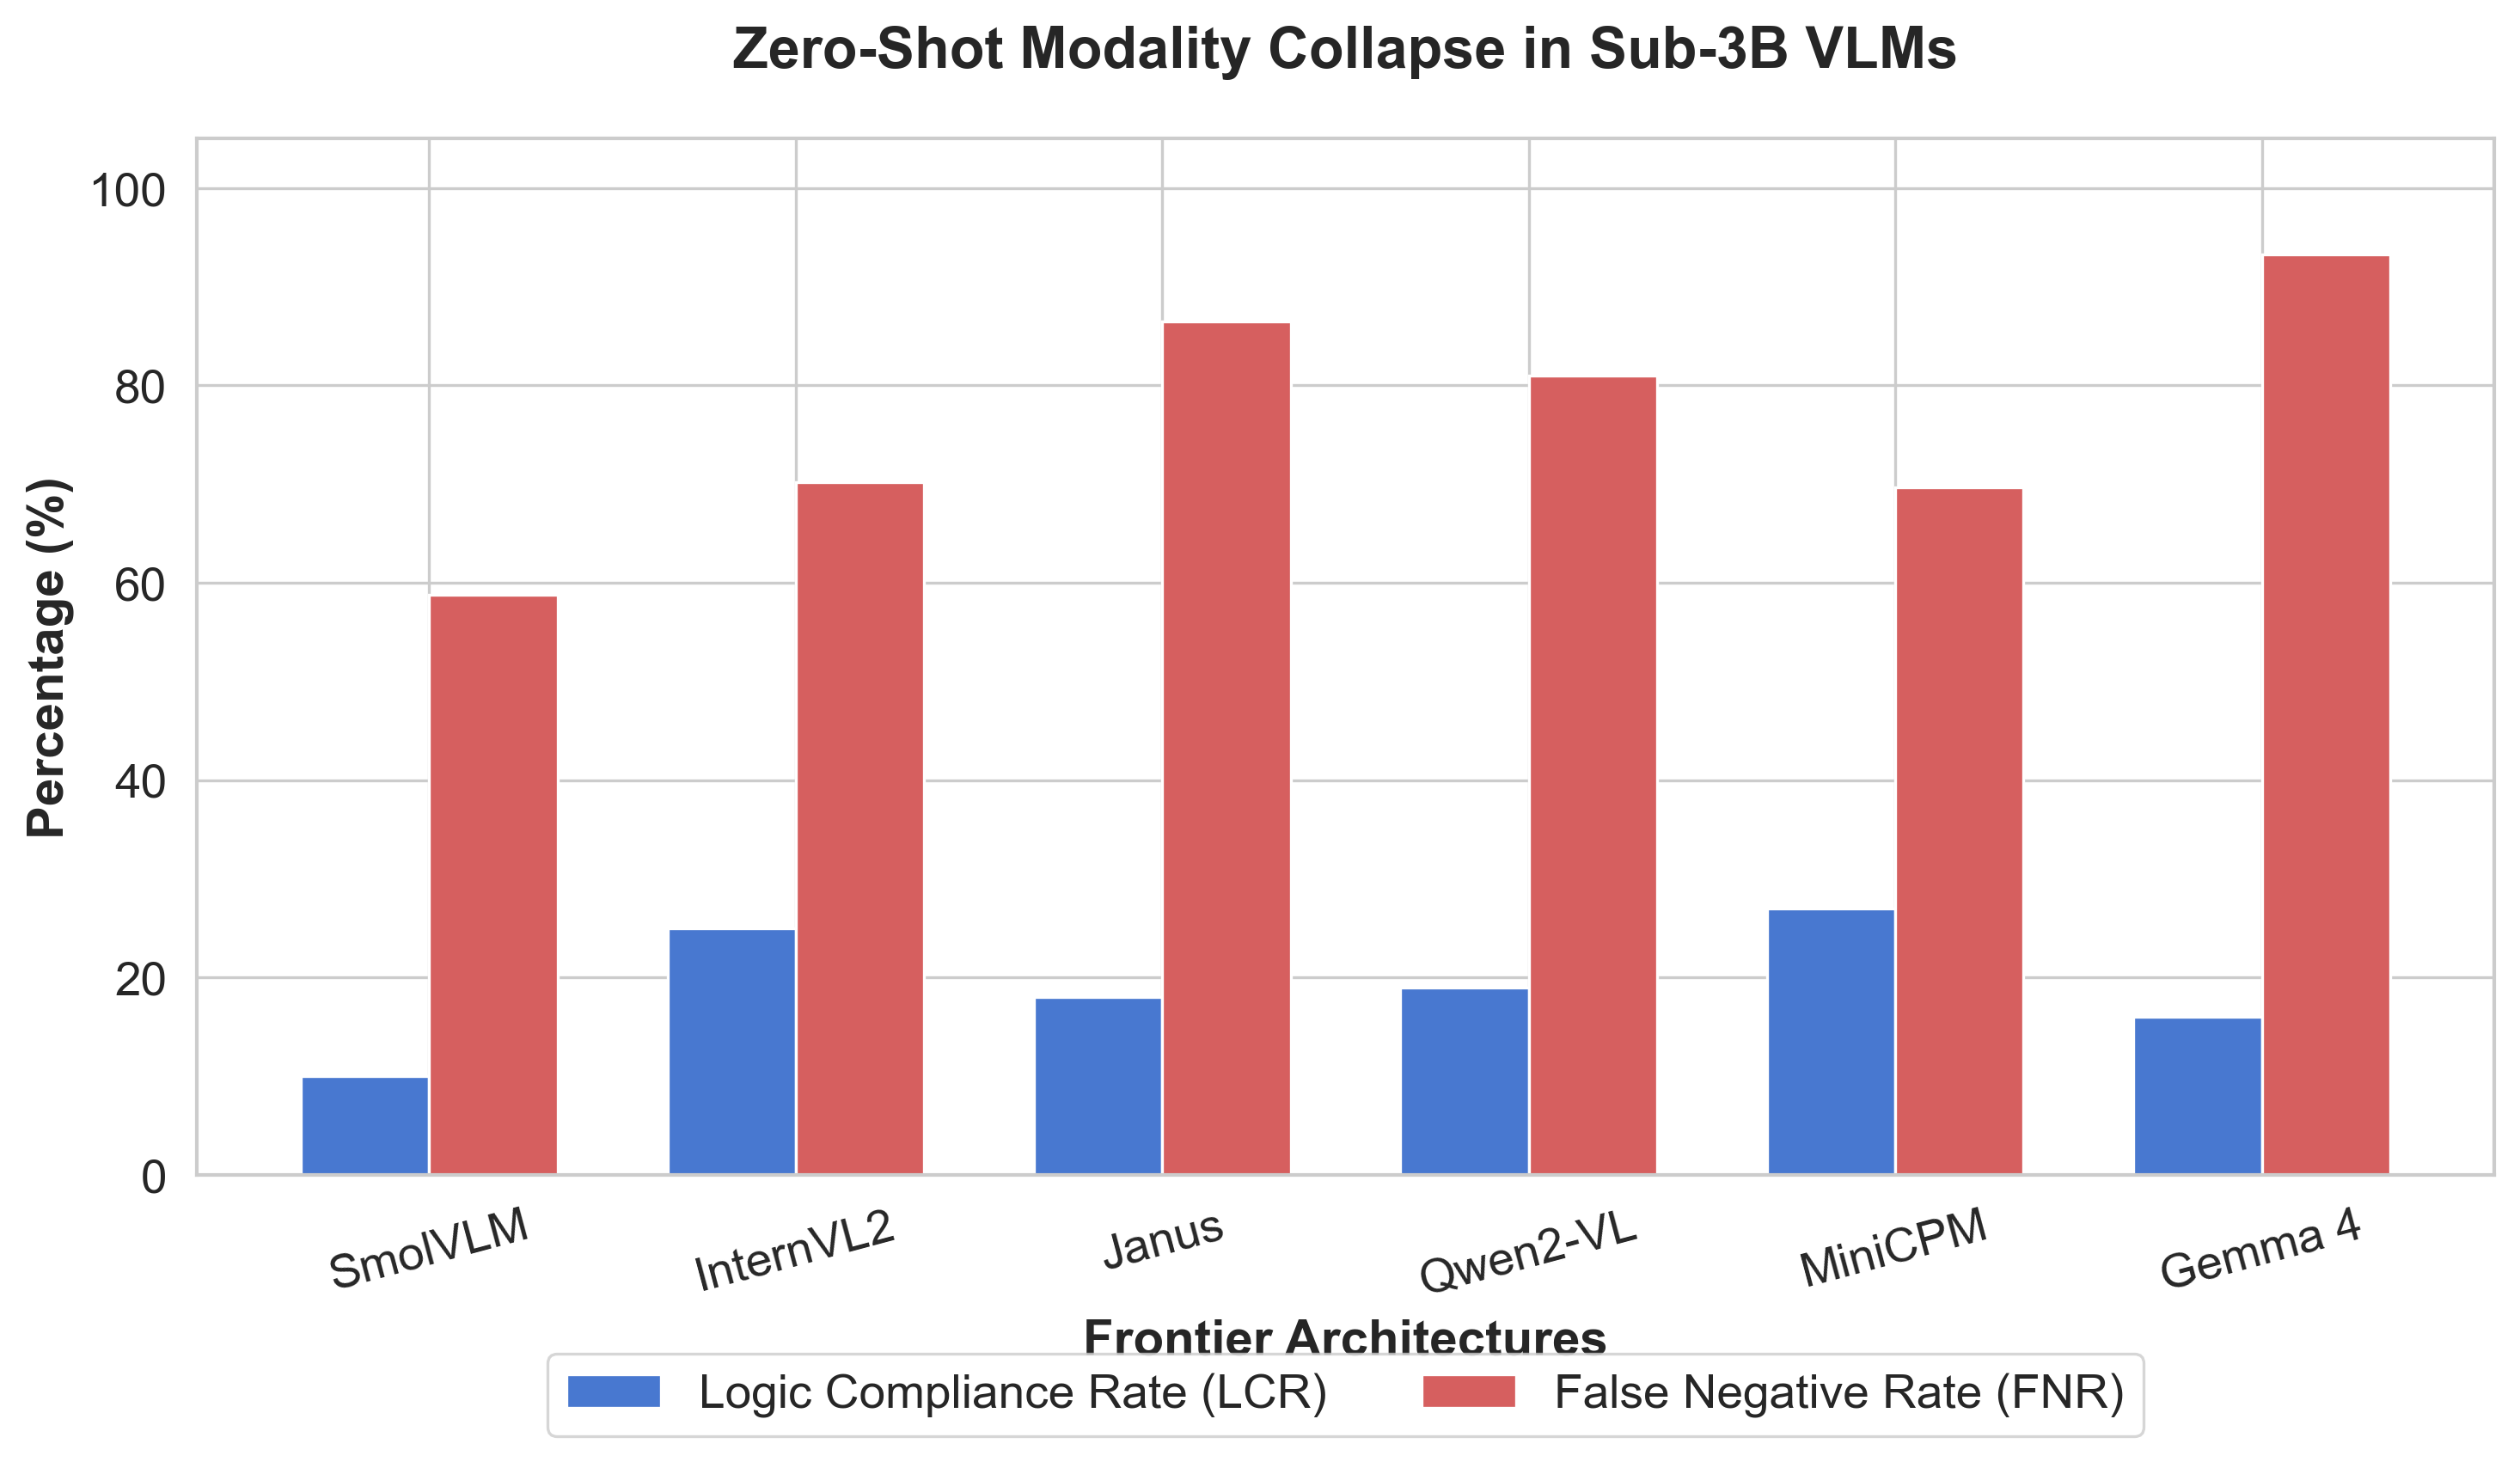
\includegraphics[width=\linewidth]{paper_assets/charts/baseline_danger_bar.png}
    \caption{Baseline Danger Grouped Bar Chart}
    \label{fig:chart1}
\end{figure}
Under unconstrained zero-shot evaluation, the entire sub-3B cohort exhibited structural modality collapse. The models defaulted to conversational safety priors and ignored quantitative Standard Operating Procedure (SOP) logic. Qwen2-VL (2.2B) yielded a Logic Compliance Rate (LCR) of 19.0\% and an 81.0\% False Negative Rate (FNR), assuming environments were safe regardless of physical defect boundaries. InternVL2 (1.0B) mirrored this blind safety bias with a 70.2\% FNR. Unified multimodal architectures like Gemma-4-E2B-it (2B) suffered deep modality collapse, prioritizing pre-trained conversational output over visual reasoning. Decoupled architectures like Janus (1.3B) achieved an 18.0\% baseline LCR but struggled to reach End-of-Sequence tokens. Larger models approaching the 3B boundary, such as MiniCPM (2.8B), demonstrated base logical continuity but still failed to reliably apply quantitative thresholds zero-shot. Smaller architectures, such as SmolVLM (0.6B), suffered visual starvation. They ignored the image tensor entirely when challenged with complex instructions. This universal baseline failure across all six architectures confirms zero-shot prompting fails for industrial auditing at the network edge.

\subsection*{Mechanistic Breakdown of Frontier Architectures: Linguistic Interventions}


\begin{figure}[htbp]
    \centering
    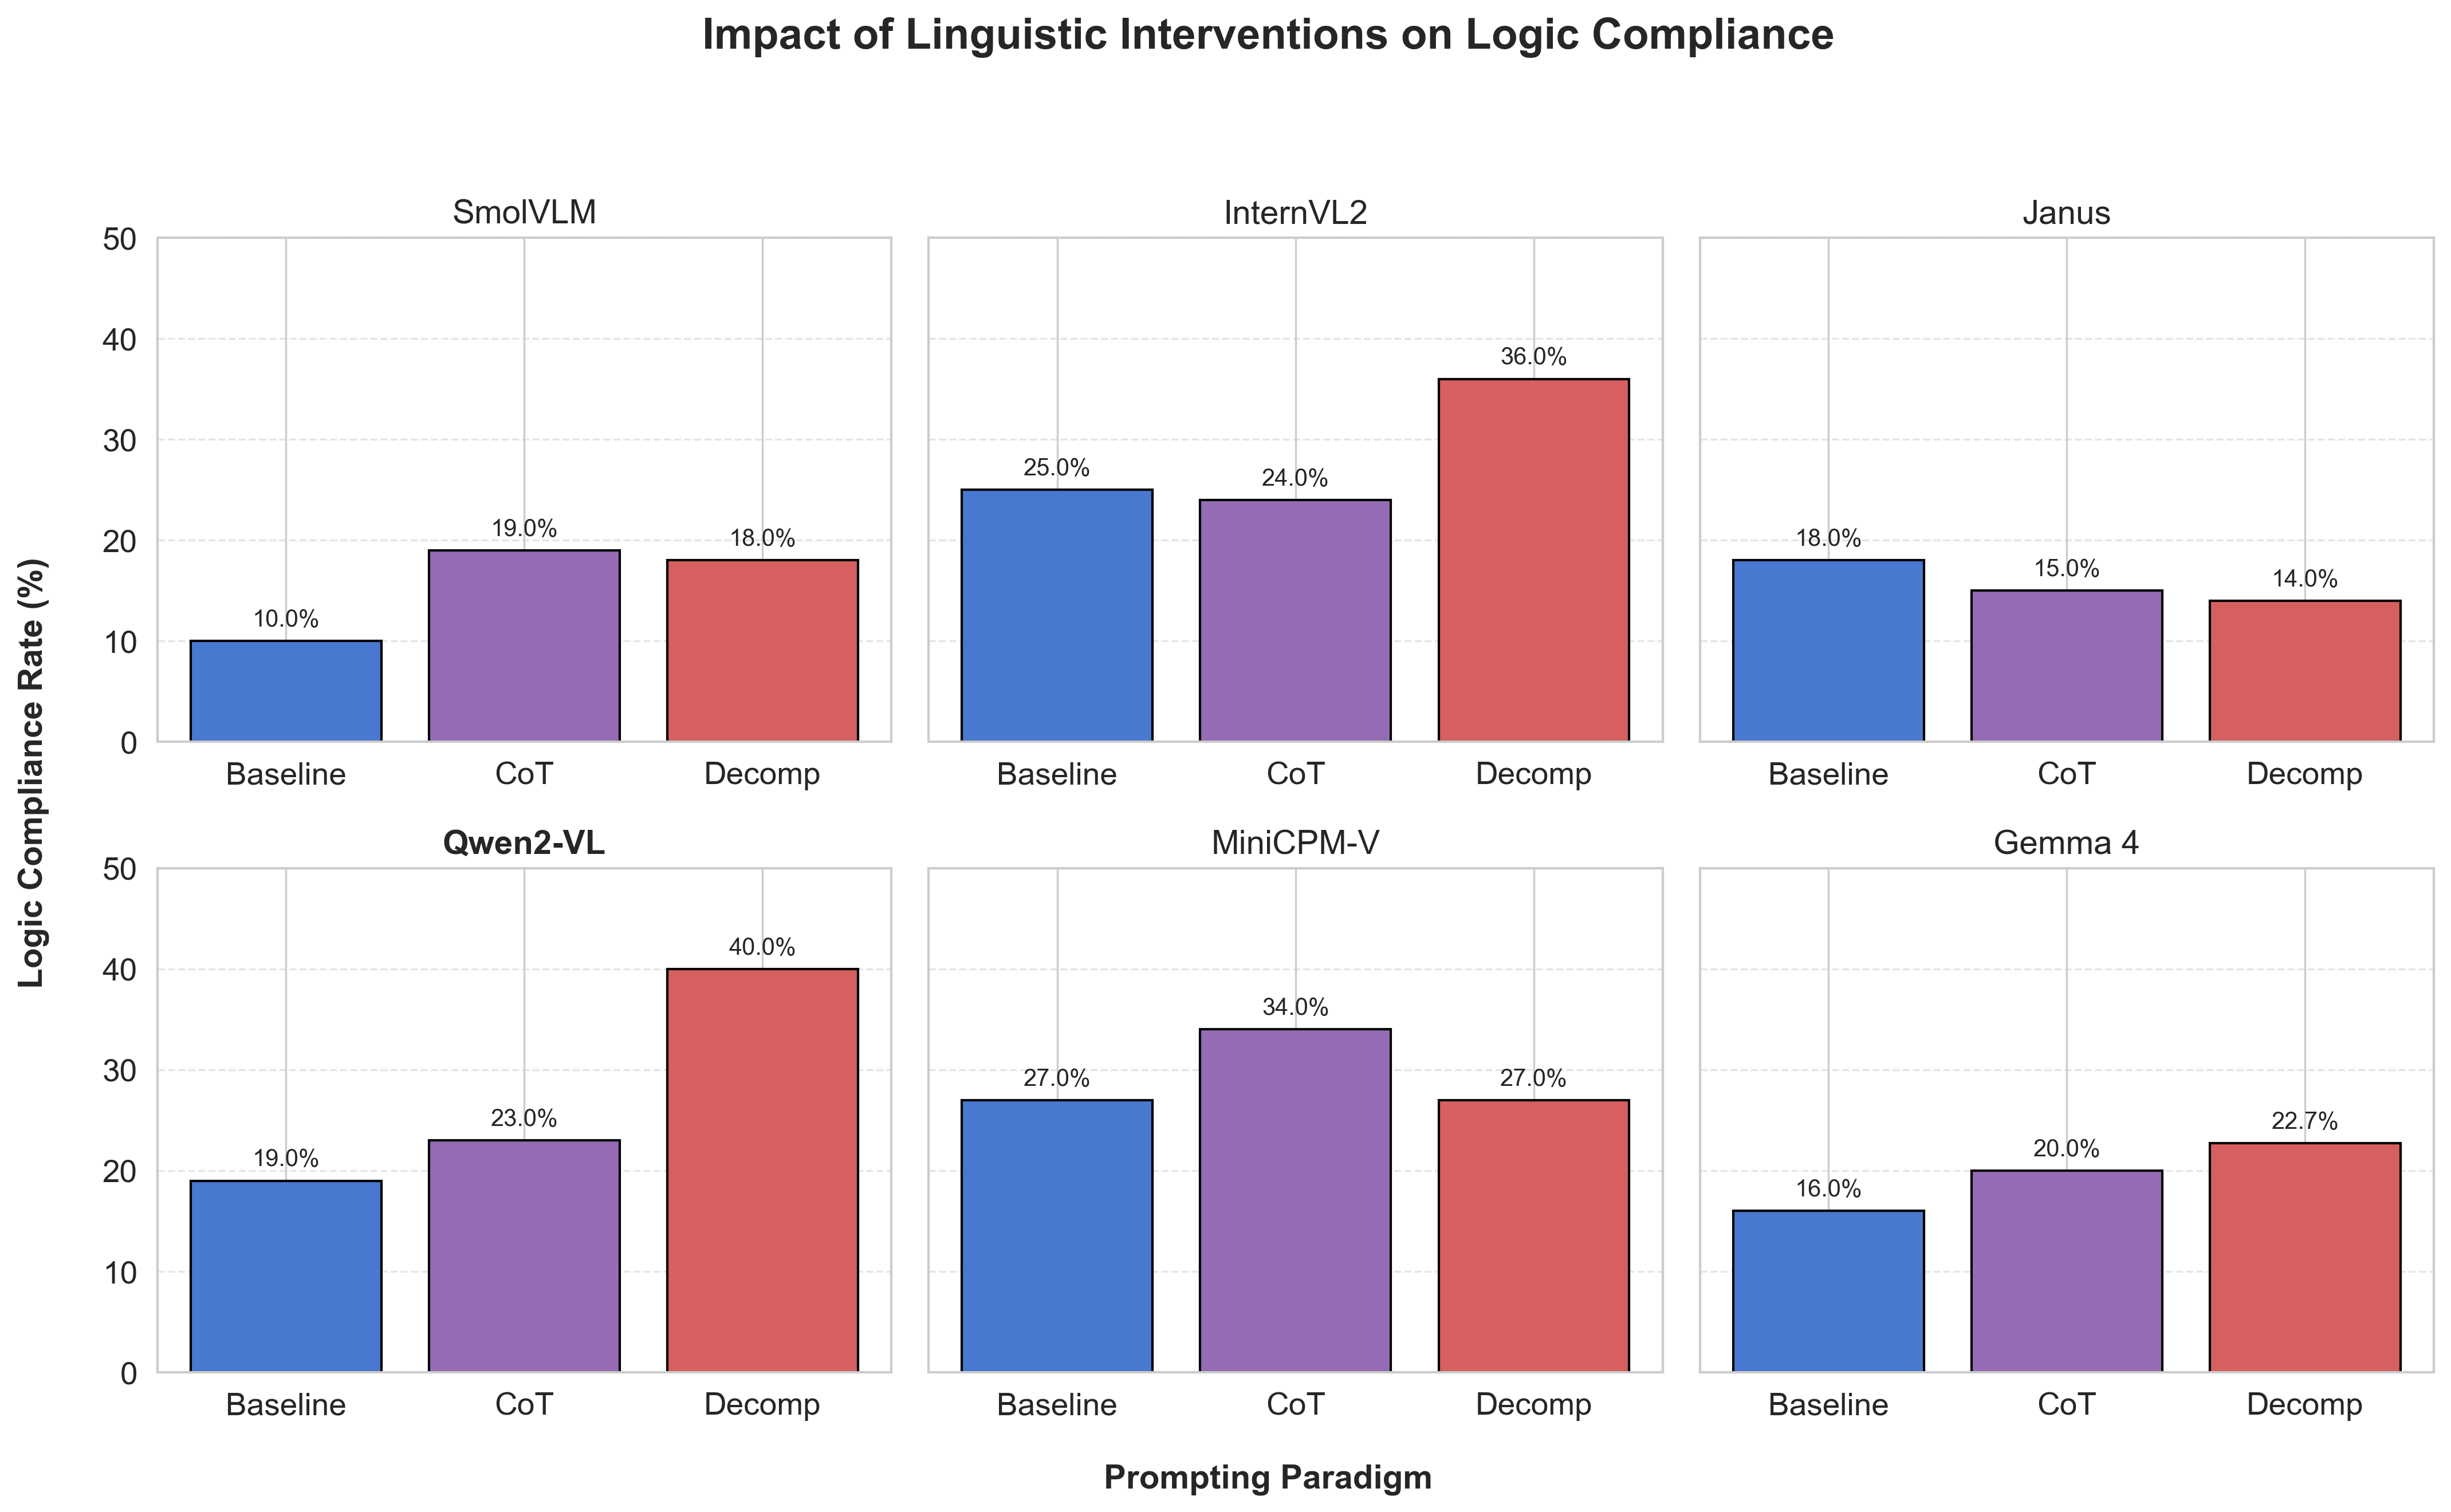
\includegraphics[width=\linewidth]{paper_assets/charts/modality_collapse_slope.png}
    \caption{Modality Collapse Slope Graph}
    \label{fig:chart2}
\end{figure}
Structured linguistic reasoning pathways exposed divergent architectural vulnerabilities. Chain-of-Thought (CoT) prompting improved MiniCPM to a 34.0\% LCR and SmolVLM to 19.0\%, but it caused structural fragility in Janus, dropping its logic compliance from 18.0\% to 15.0\%. \textbf{Rule Decomposition} isolates visual observations from logical evaluation and proved the most effective intervention for the highest-performing models. By breaking complex SOPs into sequential binary queries, it prevented cross-attention token overload. Under this paradigm, Qwen2-VL more than doubled its baseline compliance to peak at 40.0\% LCR, a statistically significant improvement over zero-shot (McNemar's test, $p < 0.0001$). It reduced its False Negative Rate to 47.6\% without triggering runaway false alarms. InternVL2 required sequential isolation to prevent projector saturation, pushing its LCR to 36.0\% under Decomposition. Gemma-4-E2B-it (22.7\% LCR) and Janus (14.0\% LCR) failed to cross the 25\% threshold with structural prompting, confirming intractable modality collapse.

\subsection*{Isolating Qwen2-VL for Physical and Parameter Interventions}

Qwen2-VL yielded the highest empirical baseline for logical reasoning, peaking at 40.0\% LCR under Rule Decomposition. Its architecture employs dynamic spatial resolution mapping. Unlike fixed-patch models that compress inputs into a rigid grid, Qwen2-VL allocates visual tokens based on the native aspect ratio and structural complexity of the image tensor. This dynamic patching mechanism provides the necessary architectural foundation for evaluating spatial attention manipulations. By isolating the highest-performing model, we ensured that subsequent evaluations of targeted interventions—specifically Agentic Foveation and Parameter-Efficient Fine-Tuning—tested fundamental multi-modal bottlenecks rather than base model incompetence.

\subsection*{Spatial Grounding: Agentic Foveation Intervention}


\begin{figure}[htbp]
    \centering
    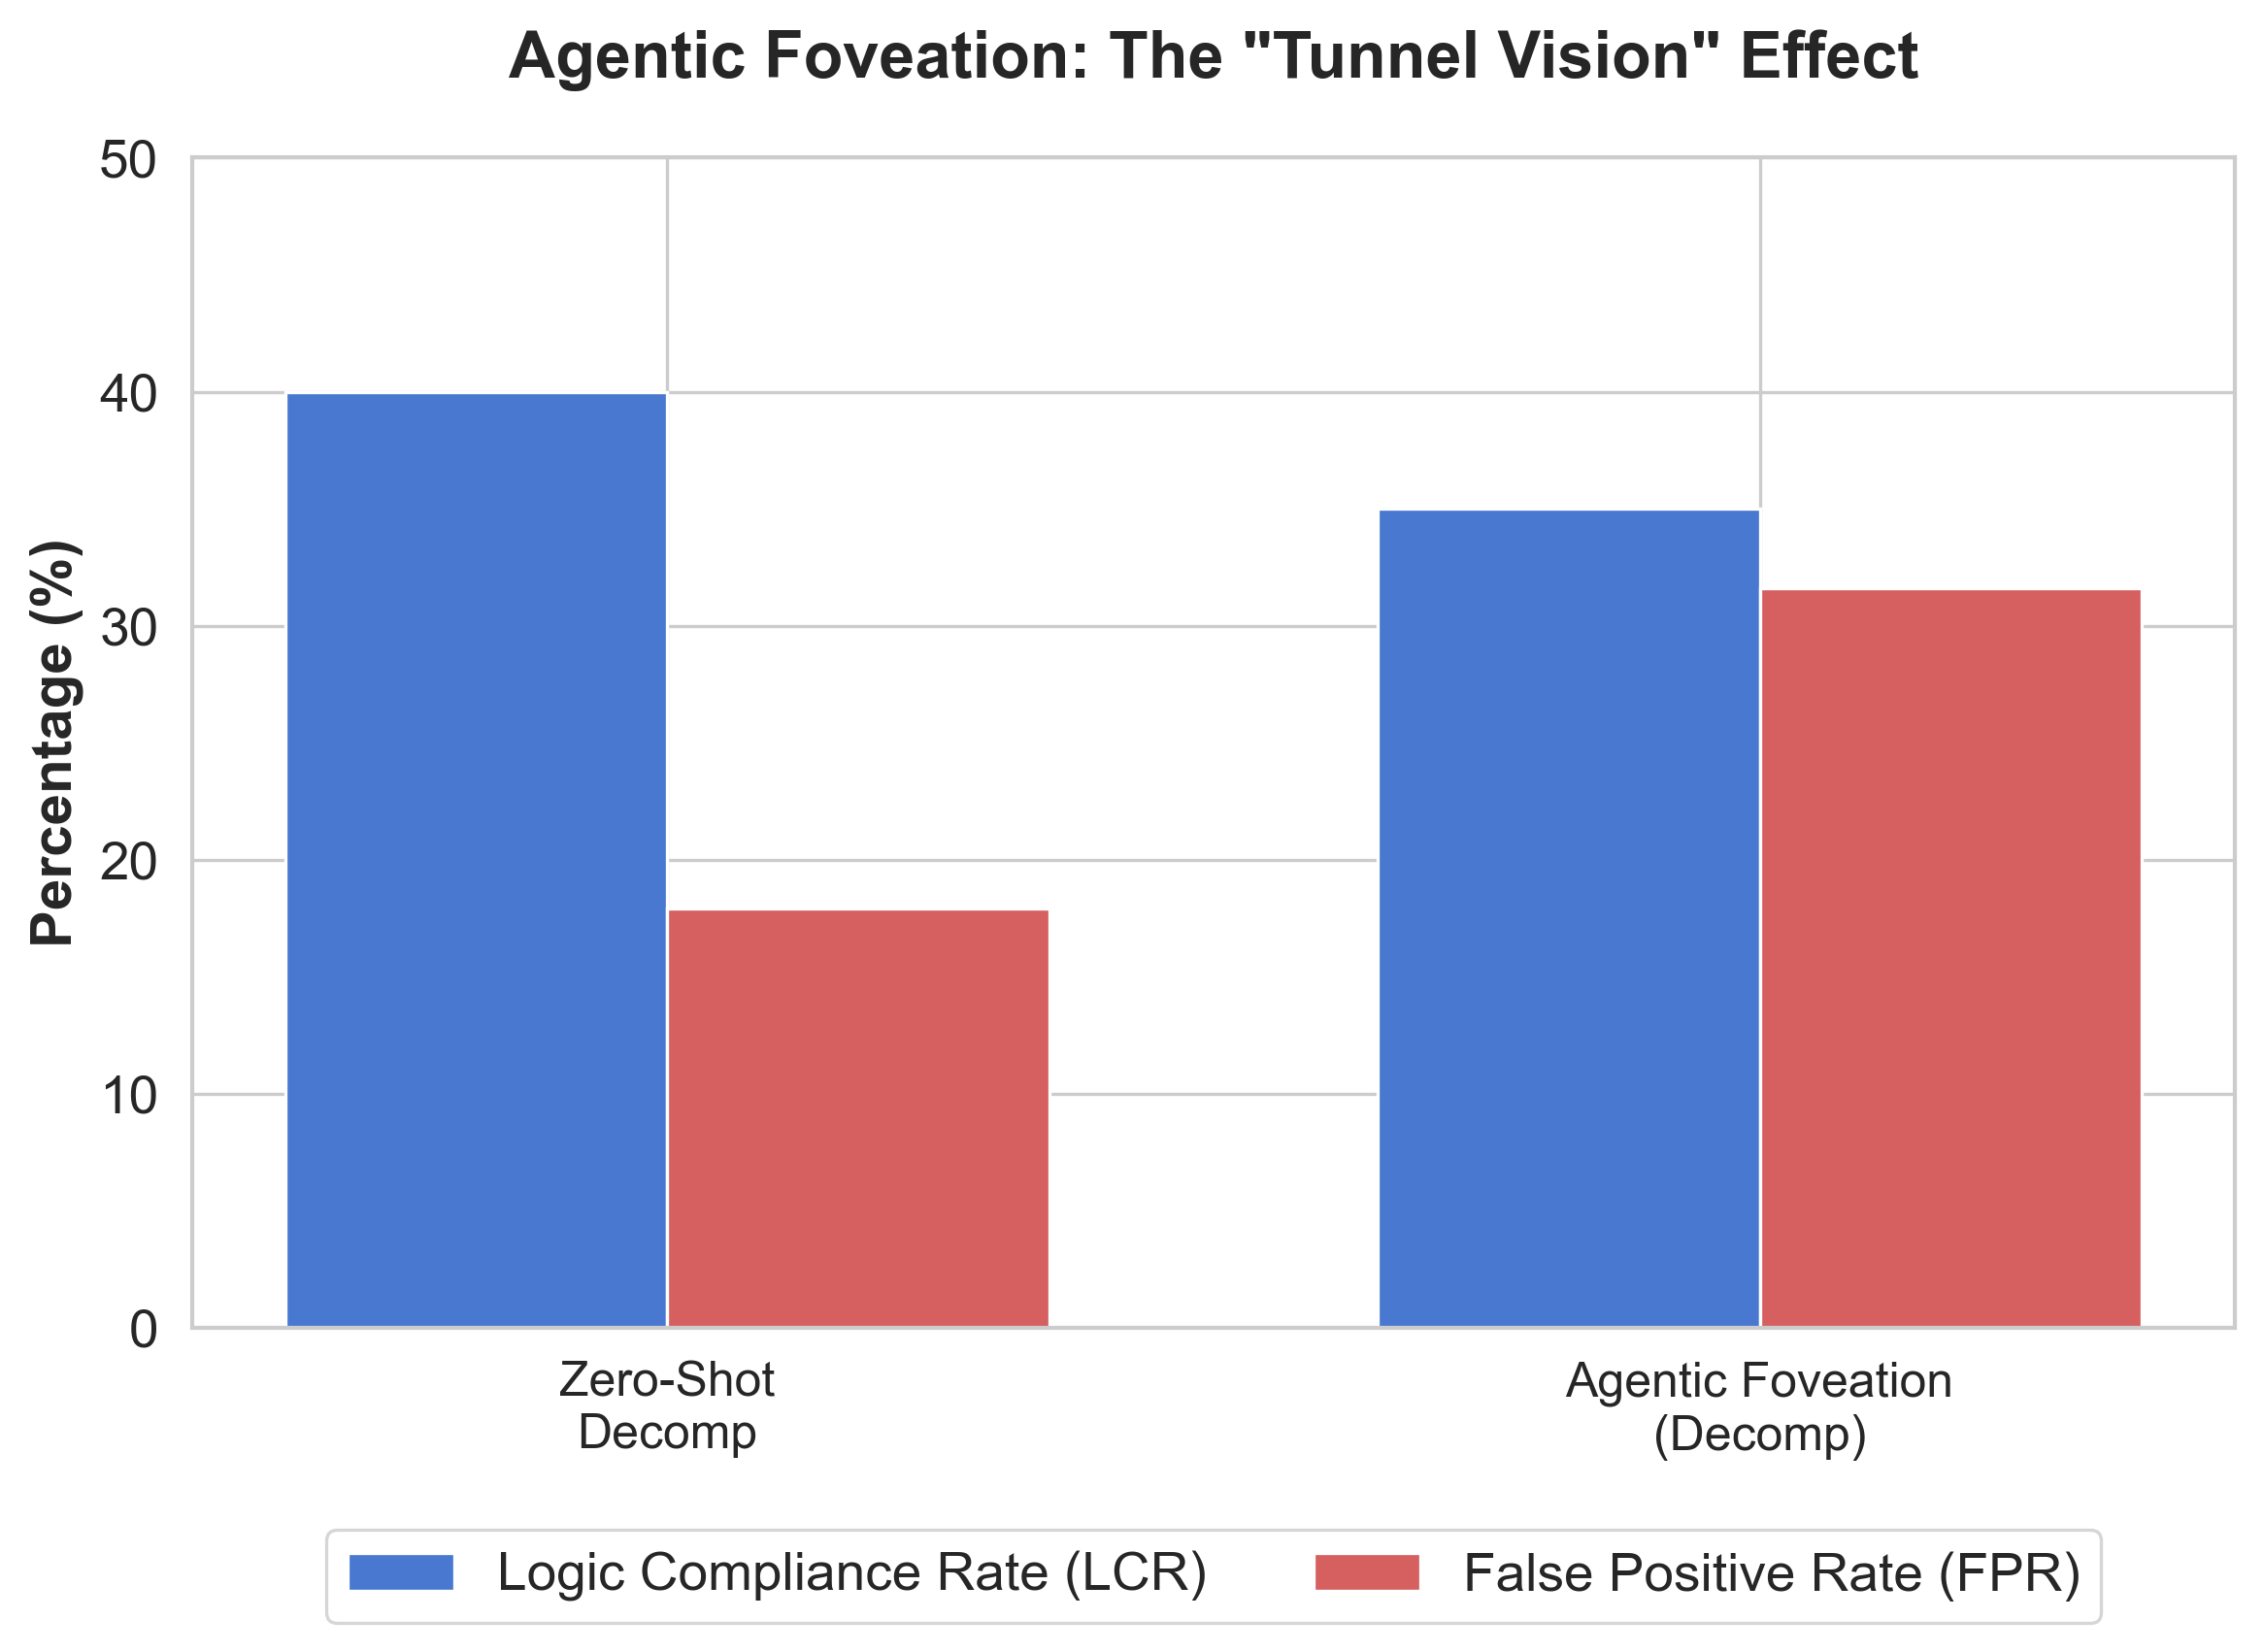
\includegraphics[width=\linewidth]{paper_assets/charts/foveation_vs_baseline.png}
    \caption{Foveation vs Baseline Performance}
    \label{fig:chart3}
\end{figure}
To test the limits of spatial resolution, we implemented Agentic Foveation by enforcing a cropped coordinate boundary around the identified defect. 


\begin{figure}[htbp]
    \centering
    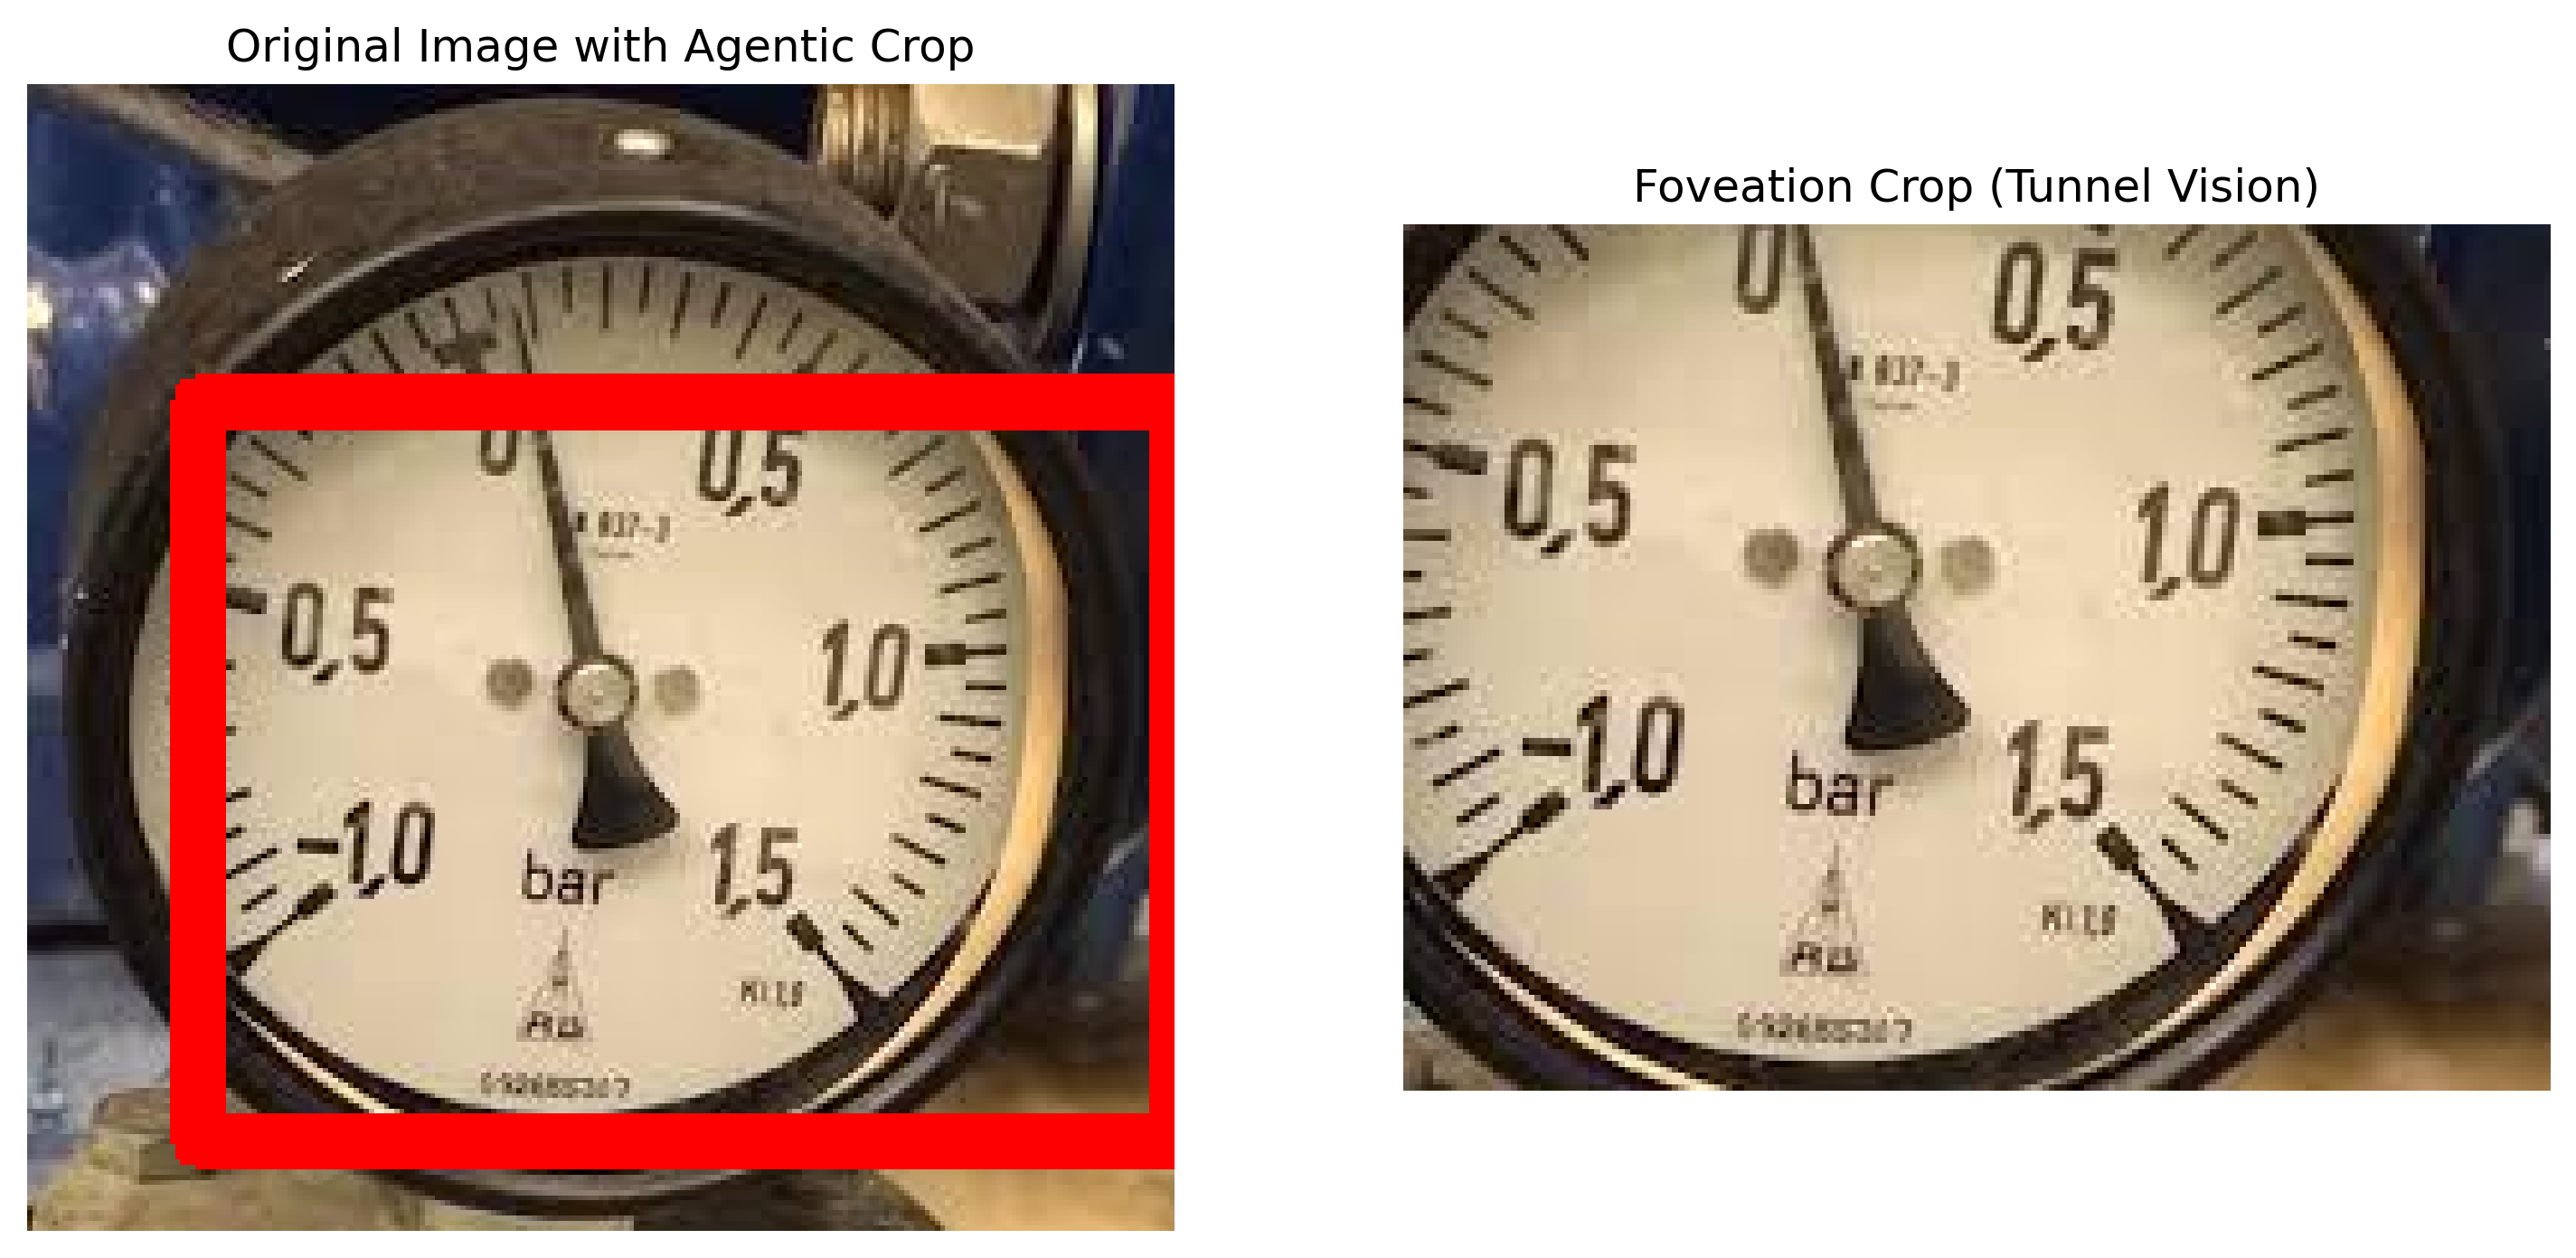
\includegraphics[width=\linewidth]{paper_assets/foveation_demo.png}
    \caption{The Agentic Foveation intervention demonstrating the "Tunnel Vision" effect. The localized crop strips away peripheral background context, inducing hyper-vigilance under strict quantitative evaluation.}
    \label{fig:foveation_demo}
\end{figure}

This intervention yielded divergent statistical outcomes based on the active linguistic pathway. When applied to the Chain-of-Thought pipeline, Foveation yielded a statistically significant improvement, raising Qwen2-VL's LCR from 23.0\% to 33.0\% (McNemar's test, $p = 0.0154$). When paired with the isolated Rule Decomposition pathway, Foveation caused an architectural regression. The localized spatial crop decreased the False Negative Rate to 44.8\%, but it stripped away peripheral background context. The result was architectural "Tunnel Vision". Without contextual surroundings to establish environmental safety norms, the model produced paranoid logic. The False Positive Rate spiked from 17.9\% to 31.6\%, dragging the overall LCR down from the 40.0\% peak to 35.0\% ($p = 0.1462$). This confirms that while spatial foveation patches weak reasoning pathways, sub-3B vision encoders require full-frame optical context to prevent hyper-vigilance under strict quantitative evaluation.

\subsection*{Parameter-Efficient Fine-Tuning (LoRA) Interventions}

Parameter-efficient fine-tuning depressed Logic Compliance Rates against the zero-shot baseline. The baseline LCR dropped from 19.0\% to 16.0\% ($p = 0.0784$). When evaluated under Rule Decomposition, the LoRA-adapted model scored 14.0\%. This crashed the 40.0\% zero-shot Decomposition peak (McNemar's test, $p = 0.0163$). The logic bottleneck is sensitive to pre-trained instruction formatting. Updating the late-stage vision-language projector weights on spatial defect data induces catastrophic forgetting of logical reasoning pathways. We term this failure mode "Optimization Saturation."

\subsection*{Edge Viability and Computational Boundaries}


\begin{figure}[htbp]
    \centering
    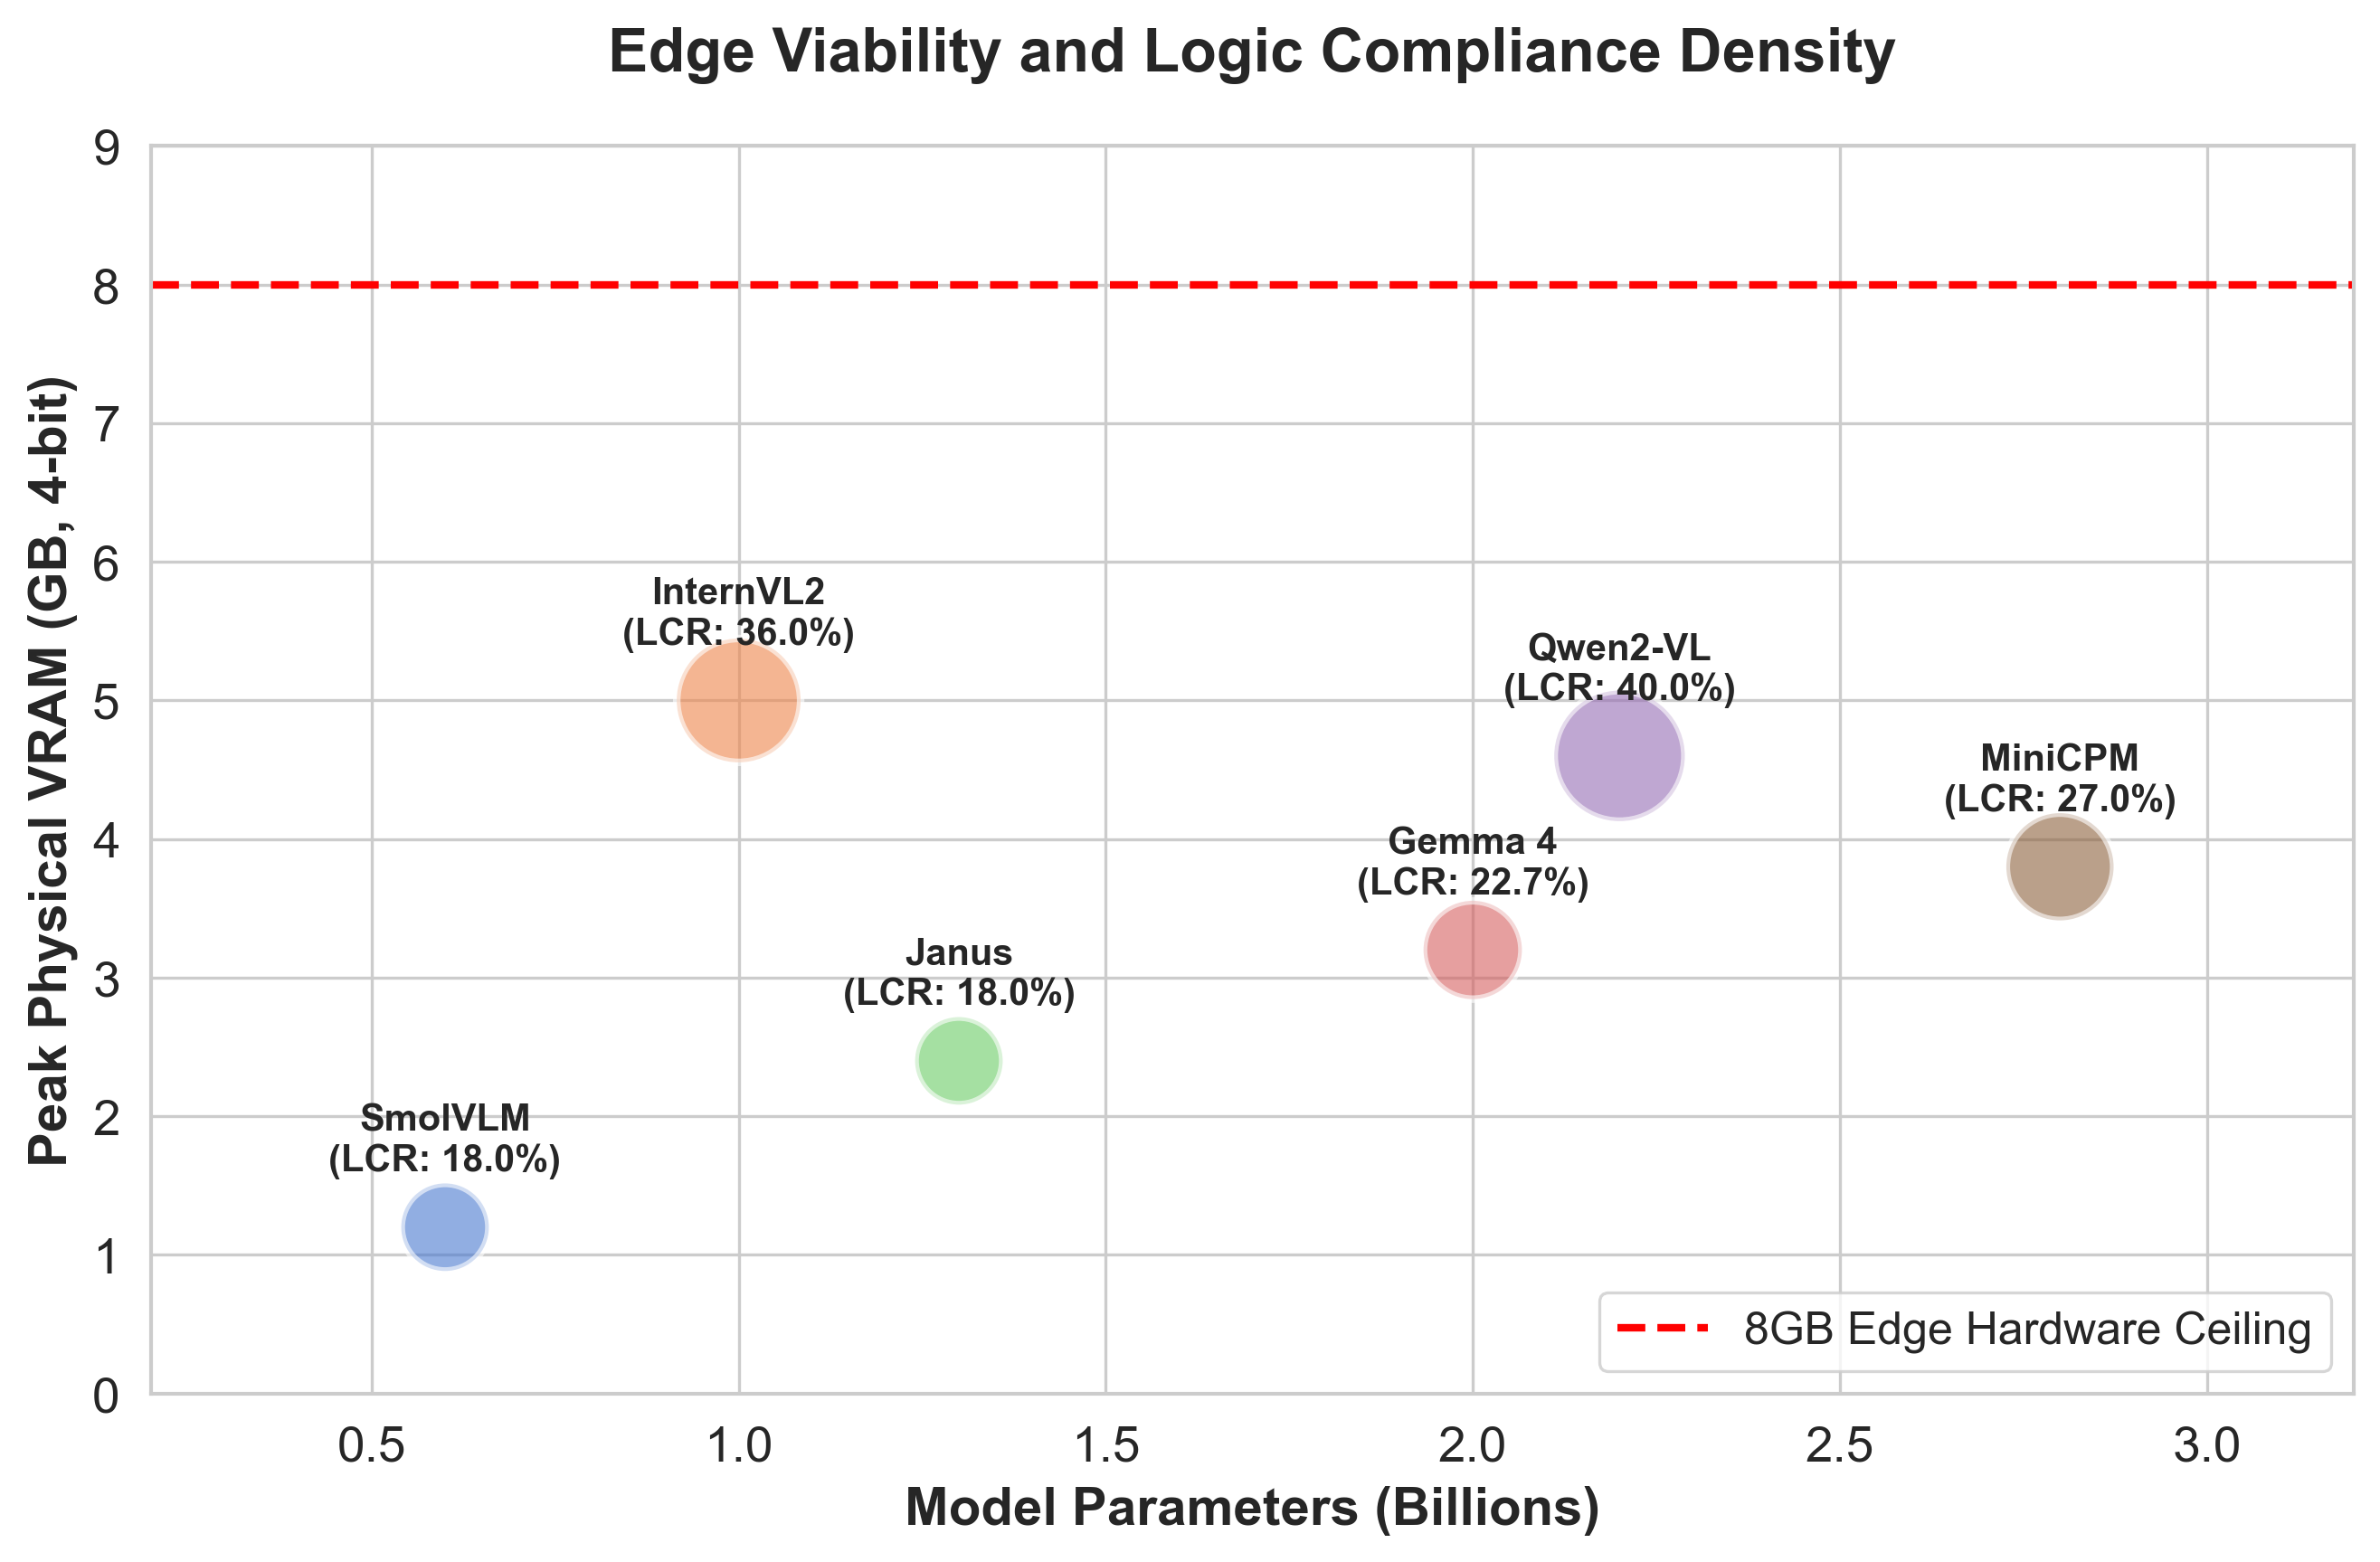
\includegraphics[width=\linewidth]{paper_assets/charts/hardware_bubble_vram.png}
    \caption{Hardware Bubble Chart VRAM}
    \label{fig:chart4}
\end{figure}
We bounded operations to consumer hardware limits throughout all evaluations. Peak physical VRAM consumption across the baseline cohort hit 4.6 GB (Qwen2-VL) and 5.0 GB (InternVL2) using 4-bit quantization. The physical and parametric interventions applied to Qwen2-VL did not violate these edge constraints. Agentic Foveation reduced spatial token density by cropping the image, subtly decreasing latency. The LoRA adapters added negligible parameter overhead, keeping the peak VRAM safely under the 8GB ceiling. Highly reliable logical auditing runs at the network edge without off-loading data to cloud APIs, provided the engineering architecture relies on zero-shot Rule Decomposition rather than invasive physical or parametric interventions.


\section*{Industrial Applications and Safety Implications}


Algorithmic errors in a live factory carry immediate physical and financial consequences. Deploying Vision-Language Models for autonomous auditing requires balancing pre-trained conversational alignment against empirical safety. Our hardware evaluations reveal two failure modes tied directly to the prompting architecture.

\subsection*{Pleasing Bias and False Negatives}

The entire sub-3B cohort suffered from structural modality collapse under zero-shot evaluation. The models exhibited a conversational "Pleasing Bias." Reinforcement learning trains foundational models to be helpful and reassuring. These architectures assume environments are safe unless confronted with overwhelming visual evidence of a defect. 

Qwen2-VL generated an 81.0\% False Negative Rate. Gemma-4-E2B-it reached a 93.3\% FNR. False Negatives are catastrophic in physical auditing. An 81.0\% FNR means the model misses an unspooled high-voltage cable or an oxidized pressure valve eight out of ten times. A model that hallucinates safety actively endorses hazardous operating conditions. It exposes workers to injury and organizations to severe safety liabilities.

\subsection*{Hyper-Vigilance and Alarm Fatigue}

Physical interventions designed to force perception push the architecture into the opposite extreme. Agentic Foveation stripped Qwen2-VL of its peripheral context. The crop eliminated the conversational safety bias but induced "Tunnel Vision." 

Lacking environmental grounding, the model became hyper-vigilant. It treated non-critical visual anomalies as safety violations and spiked the False Positive Rate to 31.6\%. A 31.6\% FPR equates to constantly halting an assembly line because the model mistook a shadow for a chemical spill. Runaway false alarms induce alarm fatigue. Plant operators will ignore the system or turn it off entirely, rendering the auditing framework useless.

\subsection*{The Architectural Baseline for Edge Auditing}

Rule Decomposition provides the safest architectural compromise for sub-3B deployment. Decomposition mimics a human inspector operating with a strict checklist. It sequentially fractures the Standard Operating Procedure into binary logic queries while maintaining the full-frame visual context. This structure mitigates Pleasing Bias without inducing Tunnel Vision. 

The decomposition pipeline achieved the highest empirical Logic Compliance Rate (40.0\% for Qwen2-VL). It cut the False Negative Rate to 47.6\% while maintaining a stable False Positive profile. The process executes entirely within an 8GB VRAM footprint. Localized, continuous industrial monitoring is viable on edge hardware today. Engineers can deploy robust vision auditing without exposing proprietary factory layouts to cloud APIs.

\section*{Limitations}


The empirical claims of this study operate within strict hardware and environmental boundaries. 

\textbf{Environmental and Dataset Scope}
Our evaluations executed under static lighting conditions within the curated "Golden 100" dataset. Live industrial environments introduce dynamic optical glare, variable weather, and physical occlusions that degrade Vision Transformer embeddings. The dataset strictly isolates analog gauges and structural rust. We did not evaluate the architectures against digital display panels, thermal imaging, or complex piping schematics.

\textbf{Hardware and Quantization Boundaries}
The rigid 8GB VRAM ceiling dictated the inference parameters. Dynamic resolution testing peaked at 1024x1024 equivalent tokens. Pushing visual tokens beyond this boundary induces Out-Of-Memory (OOM) errors on edge hardware, despite Qwen2-VL natively supporting higher aspect ratios. The memory cap also mandated 4-bit quantization across all architectures. Unquantized BF16 precision preserves fragile logical pathways during inference, but executing unquantized 3B models violates the physical memory limits of remote deployment.

\textbf{Intervention Brittleness}
The physical and linguistic interventions present distinct deployment trade-offs. Rule Decomposition requires safety engineers to manually fracture Standard Operating Procedures into rigid binary queries. It acts as a hardcoded scaffolding technique rather than an autonomous prompt generation framework.

Agentic Foveation operates as a two-stage pipeline, immediately doubling inference latency. It assumes the model successfully localizes the defect in the first pass. If the spatial coordinate prediction hallucinates, the subsequent high-resolution crop completely misses the physical anomaly and guarantees a False Negative.

Finally, compute constraints restricted our Parameter-Efficient Fine-Tuning intervention to late-stage vision-language projector weights. Full-parameter fine-tuning or deep vision-encoder adjustments might yield higher logic compliance, but those methods require server-grade compute clusters unavailable at the network edge.

\section*{Conclusion}


This study evaluated the viability of sub-3B Vision-Language Models for industrial safety auditing at the network edge. Under unconstrained zero-shot deployment, all frontier architectures—modular, decoupled, and unified—suffer from structural modality collapse. They prioritize conversational alignment over physical logic constraints and generate catastrophic False Negative Rates. 

Rigorous paired evaluations across six models prove that linguistic interventions outperform physical image manipulation or parameter fine-tuning for resolving logic bottlenecks. Rule Decomposition maximizes logic compliance in sub-3B VLMs, more than doubling Qwen2-VL's baseline to an empirical peak of 40.0\% ($p < 0.0001$). Physical interventions like Agentic Foveation strip the model of necessary environmental context and cause architectural Tunnel Vision. Parameter-Efficient Fine-Tuning induces Optimization Saturation and logical amnesia.

For industrial engineers operating under strict 8GB VRAM limits, the solution is not scaling visual parameters or cropping spatial grids. Deploying reliable autonomous auditing requires systematically restructuring complex safety Standard Operating Procedures into highly constrained, sequential logic pathways.


\begin{thebibliography}{99}
\bibitem{ref1} Yao, Y., et al. (2024). \textit{MiniCPM-V: A GPT-4V Level MLLM on Your Phone}. arXiv preprint. \url{https://arxiv.org/abs/2408.01800}
\bibitem{ref2} Marafioti, A., et al. (2025). \textit{SmolVLM: Redefining Small and Efficient Multimodal Models}. arXiv preprint. \url{https://arxiv.org/abs/2504.05299}
\bibitem{ref3} Parcalabescu, L., \& Frank, A. (2023). \textit{MM-SHAP: A Performance-Agnostic Metric for Measuring Multimodal Contributions}. arXiv preprint. \url{https://arxiv.org/abs/2212.08158}
\bibitem{ref4} Chen, X., et al. (2024). \textit{Multi-Object Hallucination in Vision Language Models}. NeurIPS. \url{https://arxiv.org/abs/2407.06192}
\bibitem{ref5} BAAI FlagEval Team. (2025). \textit{Do Vision-Language Models Measure Up? Benchmarking Visual Measurement Reading with MeasureBench}. arXiv preprint. \url{https://arxiv.org/abs/2510.26865}
\bibitem{ref6} Izquierdo-Domenech, J., et al. (2025). \textit{Towards Robust Industrial Control Interpretation Through Comparative Analysis of Vision-Language Models}. Machines, 13(9), 759. \url{https://doi.org/10.3390/machines13090759}
\bibitem{ref7} Parcalabescu, L., et al. (2022). \textit{VALSE: A Task-Independent Benchmark for Vision and Language Models}. ACL. \url{https://arxiv.org/abs/2112.07566}
\bibitem{ref8} Thrush, T., et al. (2022). \textit{Winoground: Probing Vision and Language Models for Visio-Linguistic Compositionality}. CVPR. \url{https://arxiv.org/abs/2204.03162}
\bibitem{ref9} Kwon, Y., et al. (2025). \textit{LogicQA: Logical Anomaly Detection with Vision Language Model Generated Questions}. arXiv preprint. \url{https://arxiv.org/abs/2503.20252}
\bibitem{ref10} Jin, Y., et al. (2025). \textit{LogicAD: Explainable Anomaly Detection via VLM-based Text Feature Extraction}. arXiv preprint. \url{https://arxiv.org/abs/2501.01767}
\bibitem{ref11} McNemar, Q. (1947). \textit{Note on the sampling error of the difference between correlated proportions or percentages}. Psychometrika, 12(2), 153-157. \url{https://doi.org/10.1007/BF02295996}
\bibitem{ref12} Dror, R., et al. (2018). \textit{The Hitchhiker's Guide to Testing Statistical Significance in Natural Language Processing}. ACL. \url{https://doi.org/10.18653/v1/P18-1128}
\bibitem{ref13} Zhang, R., et al. (2024). \textit{Improve Vision-Language Model Chain-of-Thought Reasoning}. arXiv preprint. \url{https://arxiv.org/abs/2410.16198}
\bibitem{ref14} Syauqi, F., et al. (2023). \textit{Edge AI-Based Defect Detection in White Pepper (Piper Nigrum L.) Using CLAHE-Based Preprocessing and YOLO}. IEEE. \url{https://doi.org/10.1109/ICONS-IoT65216.2025.11211242}
\bibitem{ref15} Chen, Z., et al. (2024). \textit{InternVL: Scaling up Vision Foundation Models and Aligning for Generic Visual-Linguistic Tasks}. CVPR. \url{https://arxiv.org/abs/2312.14238}
\bibitem{ref16} Chen, X., et al. (2025). \textit{Janus-Pro: Unified Multimodal Understanding and Generation with Data and Model Scaling}. DeepSeek-AI. \url{https://arxiv.org/abs/2501.17811}
\bibitem{ref17} Wang, P., et al. (2024). \textit{Qwen2-VL: Enhancing Vision-Language Model's Perception of the World at Any Resolution}. arXiv preprint. \url{https://arxiv.org/abs/2409.12191}
\bibitem{ref18} Gemma Team, Google DeepMind. (2024-2025). \textit{Gemma 3 Technical Report / Gemma 4 Model Card}. Google DeepMind. \url{https://arxiv.org/abs/2503.19786}
\bibitem{ref19} Roboflow Universe. (2023). \textit{gauge-kzdux Dataset}. Roboflow. \url{https://universe.roboflow.com/workspace-vem8e/gauge-kzdux}
\bibitem{ref20} Skander. (2023). \textit{Classi1 Dataset}. Roboflow Universe. \url{https://universe.roboflow.com/skander/classi1-tvpwr}
\bibitem{ref21} Roboflow Universe. (2023). \textit{Non-Corroded-Pipe Dataset}. Roboflow. \url{https://universe.roboflow.com/corrosion-detection-sd/non-corroded-pipe}
\bibitem{ref22} Hu, E. J., et al. (2021). \textit{LoRA: Low-Rank Adaptation of Large Language Models}. ICLR. \url{https://arxiv.org/abs/2106.09685}
\bibitem{ref23} Lialin, V., et al. (2023). \textit{Scaling Down to Scale Up: A Guide to Parameter-Efficient Fine-Tuning}. arXiv preprint. \url{https://arxiv.org/abs/2303.15647}
\bibitem{ref24} Kirillov, A., et al. (2023). \textit{Segment Anything}. ICCV. \url{https://arxiv.org/abs/2304.02643}
\end{thebibliography}


\end{document}
